% \documentclass[table]{beamer}
\documentclass[table,handout]{beamer}
\setbeameroption{show notes}
% \setbeameroption{hide notes}
% \setbeameroption{show only notes}
\usepackage{varwidth}

\newif\ifhide
\newif\ifpost
\newif\ifhideclicker

% \hidetrue
% \hideclickertrue
% \posttrue

\newcommand{\whiteout}[1]{\textcolor{white}{#1}}
% \newcommand{\whiteoutbox}[1]{\fcolorbox{white}{white}{\parbox{\dimexpr \linewidth-2\fboxsep-2\fboxrule}{\whiteout{#1}}}}
% \newcommand{\notebox}[1]{\fcolorbox{blue}{white}{\parbox{\dimexpr \linewidth-2\fboxsep-2\fboxrule}{#1}}}
\newcommand{\whiteoutbox}[1]{\fcolorbox{white}{white}{\parbox{\linewidth}{\whiteout{#1}}}}
\newcommand{\notebox}[1]{\fcolorbox{blue}{white}{\parbox{\linewidth}{#1}}}
\newcommand{\blankbox}[1]{\phantom{\varwidth{\linewidth}\whiteoutbox{#1}\endvarwidth}}
\newcommand{\blank}[1]{\phantom{\varwidth{\linewidth}#1\endvarwidth}}

\ifhide%
    \newcommand{\hmask}[1]{\blank{#1}}%
\else%
    \newcommand{\hmask}[1]{#1}%
\fi

\ifhide%
    \newcommand{\wout}[1]{\whiteout{#1}}%
\else%
    \newcommand{\wout}[1]{#1}%
\fi

\ifhide%
    \newcommand{\hignore}[1]{}%
\else%
    \newcommand{\hignore}[1]{#1}%
\fi

\ifpost%
    \newcommand{\nopost}[1]{}%
\else%
    \newcommand{\nopost}[1]{#1}%
\fi

\ifhideclicker%
    \newcommand{\clickerslide}[1]{\stepcounter{clickerQuestionCounter}%
        \begin{frame}[t]
            \textcolor{blue}{Q \arabic{clickerQuestionCounter}:}
        \end{frame}}
\else%
    \newcommand{\clickerslide}[1]{#1}%
\fi

\ifhide%
    \newcommand{\hidebox}[1]{\blank{#1}}%
\else%
    \newcommand{\hidebox}[1]{\notebox{#1}}%
\fi

\ifhide%
    \newcommand{\wbox}[1]{\whiteoutbox{#1}}%
\else%
    \newcommand{\wbox}[1]{\notebox{#1}}%
\fi

\ifhide%
    \newcommand{\nbox}[1]{\blankbox{#1}}%
\else%
    \newcommand{\nbox}[1]{\notebox{#1}}%
\fi

\ifhideclicker%
    \newcommand{\clickeranswer}[1]{#1}%
\else%
    \ifhide%
        \newcommand{\clickeranswer}[1]{#1}%
    \else%
        \newcommand{\clickeranswer}[1]{\textbf{\textcolor{blue}{#1}}}%
    \fi
\fi

\usepackage{beamerthemesplit}
% \usetheme{boxes}
\usetheme{Malmoe}
\usecolortheme{seahorse}
% \usecolortheme{seagull}
\usepackage{ifthen}
\usepackage{xspace}
\usepackage{multirow}
\usepackage{multicol}
\usepackage{booktabs}
\usepackage{xcolor}
\usepackage{wasysym}
\usepackage{comment}
\usepackage{hyperref}
\hypersetup{pdfborder={0 0 0}, colorlinks=true, urlcolor=blue, linkcolor=blue, citecolor=blue}
\usepackage{changepage}
\usepackage[compatibility=false]{caption}
\captionsetup[figure]{font=scriptsize, labelformat=empty, textformat=simple, justification=centering, skip=2pt}
\usepackage{tikz}
\usetikzlibrary{trees,calc,backgrounds}

\usepackage[bibstyle=joaks-slides,maxcitenames=3,mincitenames=1,backend=biber]{biblatex}

\newrobustcmd*{\shortfullcite}{\AtNextCite{\renewbibmacro{title}{}\renewbibmacro{in:}{}\renewbibmacro{number}{}}\fullcite}

\newrobustcmd*{\footlessfullcite}{\AtNextCite{\renewbibmacro{title}{}\renewbibmacro{in:}{}}\footfullcite}

% Make all footnotes smaller
% \renewcommand{\footnotesize}{\scriptsize}

\definecolor{myGray}{gray}{0.9}
\colorlet{rowred}{red!30!white}

\setbeamertemplate{blocks}[rounded][shadow=true]

\setbeamercolor{defaultcolor}{bg=structure!30!normal text.bg,fg=black}
\setbeamercolor{block body}{bg=structure!30!normal text.bg,fg=black}
\setbeamercolor{block title}{bg=structure!50!normal text.bg,fg=black}

\newenvironment<>{varblock}[2][\textwidth]{%
  \setlength{\textwidth}{#1}
  \begin{actionenv}#3%
    \def\insertblocktitle{#2}%
    \par%
    \usebeamertemplate{block begin}}
  {\par%
    \usebeamertemplate{block end}%
  \end{actionenv}}

\newenvironment{displaybox}[1][\textwidth]
{
    \centerline\bgroup\hfill
    \begin{beamerboxesrounded}[lower=defaultcolor,shadow=true,width=#1]{}
}
{
    \end{beamerboxesrounded}\hfill\egroup
}

\newenvironment{onlinebox}[1][4cm]
{
    \newbox\mybox
    \newdimen\myboxht
    \setbox\mybox\hbox\bgroup%
        \begin{beamerboxesrounded}[lower=defaultcolor,shadow=true,width=#1]{}
    \centering
}
{
    \end{beamerboxesrounded}\egroup
    \myboxht\ht\mybox
    \raisebox{-0.25\myboxht}{\usebox\mybox}\hspace{2pt}
}

\newenvironment{mydescription}{
    \begin{description}
        \setlength{\leftskip}{-1.5cm}}
    {\end{description}}

\newenvironment{myitemize}{
    \begin{itemize}
        \setlength{\leftskip}{-.3cm}}
    {\end{itemize}}

% footnote without a marker
\newcommand\barefootnote[1]{%
  \begingroup
  \renewcommand\thefootnote{}\footnote{#1}%
  \addtocounter{footnote}{-1}%
  \endgroup
}

% define formatting for footer
\newcommand{\myfootline}{%
    {\it
    \insertshorttitle
    \hspace*{\fill} 
    \insertshortauthor, \insertshortinstitute
    % \ifx\insertsubtitle\@empty\else, \insertshortsubtitle\fi
    \hspace*{\fill}
    \insertframenumber/\inserttotalframenumber}}

% set up footer
\setbeamertemplate{footline}{%
    \usebeamerfont{structure}
    \begin{beamercolorbox}[wd=\paperwidth,ht=2.25ex,dp=1ex]{frametitle}%
        % \Tiny\hspace*{4mm}\myfootline\hspace{4mm}
        \tiny\hspace*{4mm}\myfootline\hspace{4mm}
    \end{beamercolorbox}}

% remove navigation bar
\beamertemplatenavigationsymbolsempty

\makeatletter
    \newenvironment{noheadline}{
        \setbeamertemplate{headline}[default]
        \def\beamer@entrycode{\vspace*{-\headheight}}
    }{}
\makeatother

\newcounter{clickerQuestionCounter}
\ifhideclicker%
\newenvironment{clickerquestion}
{ \stepcounter{clickerQuestionCounter}
  \begin{enumerate}[Q \arabic{clickerQuestionCounter}:]\color{white} }
{ \end{enumerate} }
\else%
\newenvironment{clickerquestion}
{ \stepcounter{clickerQuestionCounter}
  \begin{enumerate}[Q \arabic{clickerQuestionCounter}:] }
{ \end{enumerate} }
\fi

\ifhideclicker%
\newenvironment{clickeroptions}
{ \begin{enumerate}[\begingroup\color{white} 1)\endgroup]\color{white} }
{ \end{enumerate} }
\else%
\newenvironment{clickeroptions}
{ \begin{enumerate}[\begingroup\color{red} 1)\endgroup] }
{ \end{enumerate} }
\fi


\tikzstyle{centered} = [align=center, text centered, font=\sffamily\bfseries]
\tikzstyle{skip} = [centered, inner sep=0pt, fill]
\tikzstyle{empty} = [centered, inner sep=0pt]
\tikzstyle{inode} = [centered, circle, minimum width=4pt, fill=black, inner sep=0pt]
\tikzstyle{tnode} = [centered, circle, inner sep=1pt]
\tikzset{
  % edge styles
  level distance=10mm,
  mate/.style={edge from parent/.style={draw,distance=3pt}},
  mleft/.style={grow=left, level distance=10mm, edge from parent path={(\tikzparentnode.west)--(\tikzchildnode.east)}},
  mright/.style={grow=right, level distance=10mm, edge from parent path={(\tikzparentnode.east)--(\tikzchildnode.west)}},
  % node styles
  male/.style={rectangle,minimum size=4mm,fill=gray!80},
  female/.style={circle,minimum size=4mm,fill=gray!80},
  amale/.style={male,fill=red},
  afemale/.style={female,fill=red},
}

\newcommand{\highlight}[1]{\textcolor{violet}{\textit{\textbf{#1}}}}
\newcommand{\super}[1]{\ensuremath{^{\textrm{\sffamily #1}}}}
\newcommand{\sub}[1]{\ensuremath{_{\textrm{\sffamily #1}}}}
\newcommand{\dC}{\ensuremath{^\circ{\textrm{C}}}}
\newcommand{\tb}{\hspace{2em}}
\providecommand{\e}[1]{\ensuremath{\times 10^{#1}}}
\newcommand{\myHangIndent}{\hangindent=5mm}

\newcommand{\spp}[1]{\textit{#1}}

\newcommand\mybullet{\leavevmode%
\usebeamertemplate{itemize item}\hspace{.5em}}

\makeatletter
\newcommand*{\rom}[1]{\expandafter\@slowromancap\romannumeral #1@}
\makeatother

\newcommand{\blankslide}{{\setbeamercolor{background canvas}{bg=black}
\setbeamercolor{whitetext}{fg=white}
\begin{frame}<handout:0>[plain]
\end{frame}}}

\newcommand{\whiteslide}{
\begin{frame}<handout:0>[plain]
\end{frame}}

\newcommand{\f}[1]{\ensuremath{F_{#1}}}
\newcommand{\x}[1]{X\ensuremath{^{#1}}}
\newcommand{\y}[1]{Y\ensuremath{^{#1}}}

% Population growth macros
\newcommand{\popsize}[1]{\ensuremath{N_{#1}}}
\newcommand{\popgrowthratediscrete}[1]{\ensuremath{\lambda_{#1}}}
\newcommand{\popgrowthrate}[1]{\ensuremath{r_{#1}}}
\newcommand{\ptime}{\ensuremath{t}\xspace}

\tikzset{hide on/.code={\only<#1>{\color{white}}}}
\tikzset{
    invisible/.style={opacity=0},
    visible on/.style={alt={#1{}{invisible}}},
    alt/.code args={<#1>#2#3}{%
        \alt<#1>{\pgfkeysalso{#2}}{\pgfkeysalso{#3}}
        % \pgfkeysalso doesn't change the path
    },
}

\bibliography{../bib/references}
\author[J.\ Oaks]{
    %Jamie R.\ Oaks\inst{1}
    Jamie R.\ Oaks
}
\institute[BIOL 180]{
    \inst{}%
        BIOL 180: Introductory Biology
}



\title[Professioinal Development II]{Professioinal Development II: Career
    planning (and graduate/professional school preparation)}
% \date{\today}
\date{April 16, 2015}

\begin{document}

\begin{noheadline}
\maketitle
\end{noheadline}

\nopost{
\begin{noheadline}
\begin{frame}[c]
    \vspace{-1.3cm}
    \begin{center} 
        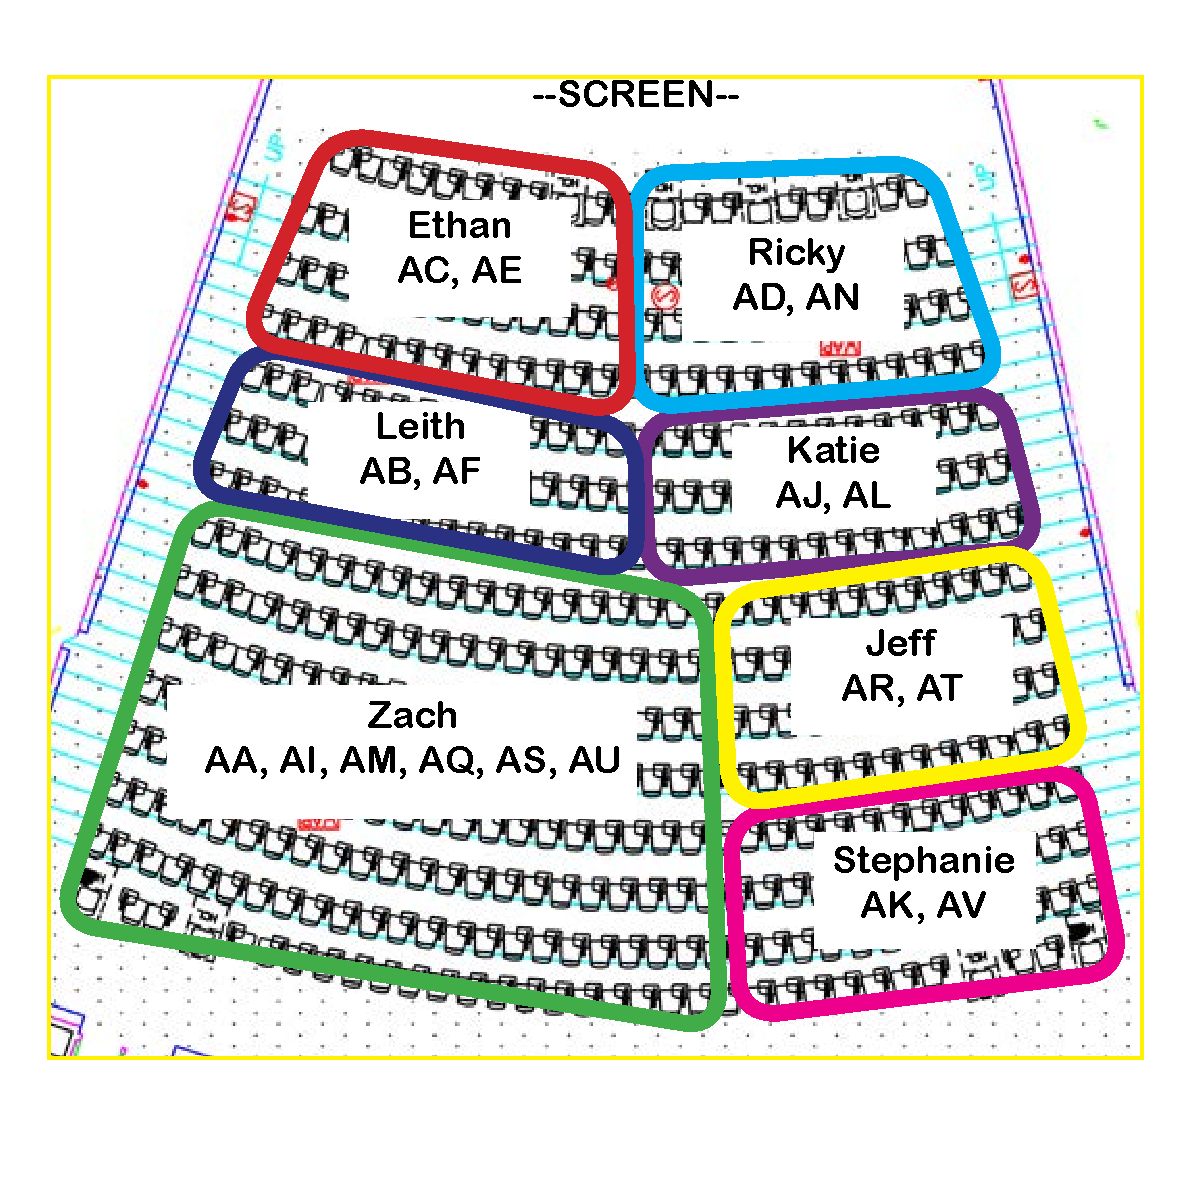
\includegraphics[height=1.3\textheight]{../images/seating-chart.pdf}
    \end{center}
\end{frame}
\end{noheadline}
}

\begin{noheadline}
\begin{frame}
\frametitle{Today's questions:}
\tableofcontents[subsectionstyle=hide]
\end{frame}
\end{noheadline}


\section{What careers can you pursue with a biology-related degree?}

\clickerslide{
\begin{noheadline}
\begin{frame}[t]
    \textcolor{blue}{Q 1:} What is the \#1 career choice of Bio 180 students?
    \begin{table}%[htbp]
        \begin{flushleft}
        \begin{tabular}{ l l r }
            \textcolor{red}{1)} & Dentist (DDS)                    &  \\
            \textcolor{red}{2)} & Ecology/conservation             &  \\
            \textcolor{red}{3)} & Law/business                     &  \\
            \textcolor{red}{4)} & Pharmacy                         &  \\
            \textcolor{red}{5)} & PT/OT/allied health              &  \\
            \textcolor{red}{6)} & Physician (MD)                   &  \\
            \textcolor{red}{7)} & Plant science                    &  \\
            \textcolor{red}{8)} & Public/global health             &  \\
            \textcolor{red}{9)} & Research: biomed/biotech         &  \\
            \textcolor{red}{10)} & Teaching                        &  \\
            \textcolor{red}{11)} & Undecided                       &  \\
            \textcolor{red}{12)} & Other                           &  \\
            \textcolor{red}{13)} & Computer Science/Engineering    &  \\
            \textcolor{red}{14)} & Veterinary Medicine             &  \\
        \end{tabular}
        \end{flushleft}
    \end{table}
\end{frame}
\end{noheadline}
}

\clickerslide{
\begin{noheadline}
\begin{frame}[t]
    \textcolor{blue}{Q 2:} What is the LEAST popular choice of Bio 180 students?
    \begin{table}%[htbp]
        \begin{flushleft}
        \begin{tabular}{ l l r }
            \textcolor{red}{1)} & Dentist (DDS)                    & \uncover<2->{5.5\%} \\
            \textcolor{red}{2)} & Ecology/conservation             & \uncover<3->{7.1\%} \\
            \textcolor{red}{3)} & Law/business                     & \uncover<4->{2.9\%} \\
            \textcolor{red}{4)} & Pharmacy                         & \uncover<5->{6.4\%} \\
            \textcolor{red}{5)} & PT/OT/allied health              & \uncover<6->{9.5\%} \\
            \textcolor{red}{6)} & Physician (MD)                   & \uncover<7->{31.2\%} \\
            \textcolor{red}{7)} & Plant science                    & \uncover<8->{1.0\%} \\
            \textcolor{red}{8)} & Public/global health             & \uncover<9->{5.4\%} \\
            \textcolor{red}{9)} & Research: biomed/biotech         & \uncover<10->{12.3\%} \\
            \textcolor{red}{10)} & Teaching                        & \uncover<11->{1.2\%} \\
            \textcolor{red}{11)} & Undecided                       & \uncover<12->{6.9\%} \\
            \textcolor{red}{12)} & Other                           & \uncover<13->{4.0\%} \\
            \textcolor{red}{13)} & Computer Science/Engineering    & \uncover<14->{5.3\%} \\
            \textcolor{red}{14)} & Veterinary Medicine             & \uncover<15->{1.2\%} \\
        \end{tabular}
        \end{flushleft}
    \end{table}

    \note[item]{Data from Fall 2014}
    \note[item]{70.2\% clinical medicine or clinical research}
    \note[item]{Irony: \#1 public health issue in developed countries is
        obesity, and \#1 issue in developing countries is food security}
    \note[item]{The biggest challenge in health is food, and no one wants to
        work on it}
    \note[item]{Demand for biomed research is very low\ldots crisis with so
        many in/entering field}
    \note[item]{Demand for plant researchers expected to be extremely high}
\end{frame}
\end{noheadline}
}

{
\usebackgroundtemplate{
\includegraphics[page=5,width=\paperwidth]{./scotts-slides.pdf}}
\begin{frame}[plain]
    \note[item]{What do Husky bio grads actually do?}
\end{frame}
}
{
\usebackgroundtemplate{
\includegraphics[page=6,width=\paperwidth]{./scotts-slides.pdf}}
\begin{frame}[plain]
\end{frame}
}
{
\usebackgroundtemplate{
\includegraphics[page=7,width=\paperwidth]{./scotts-slides.pdf}}
\begin{frame}[plain]
\end{frame}
}
{
\usebackgroundtemplate{
\includegraphics[page=8,width=\paperwidth]{./scotts-slides.pdf}}
\begin{frame}[plain]
\end{frame}
}
{
\usebackgroundtemplate{
\includegraphics[page=9,width=\paperwidth]{./scotts-slides.pdf}}
\begin{frame}[plain]
\end{frame}
}
{
\usebackgroundtemplate{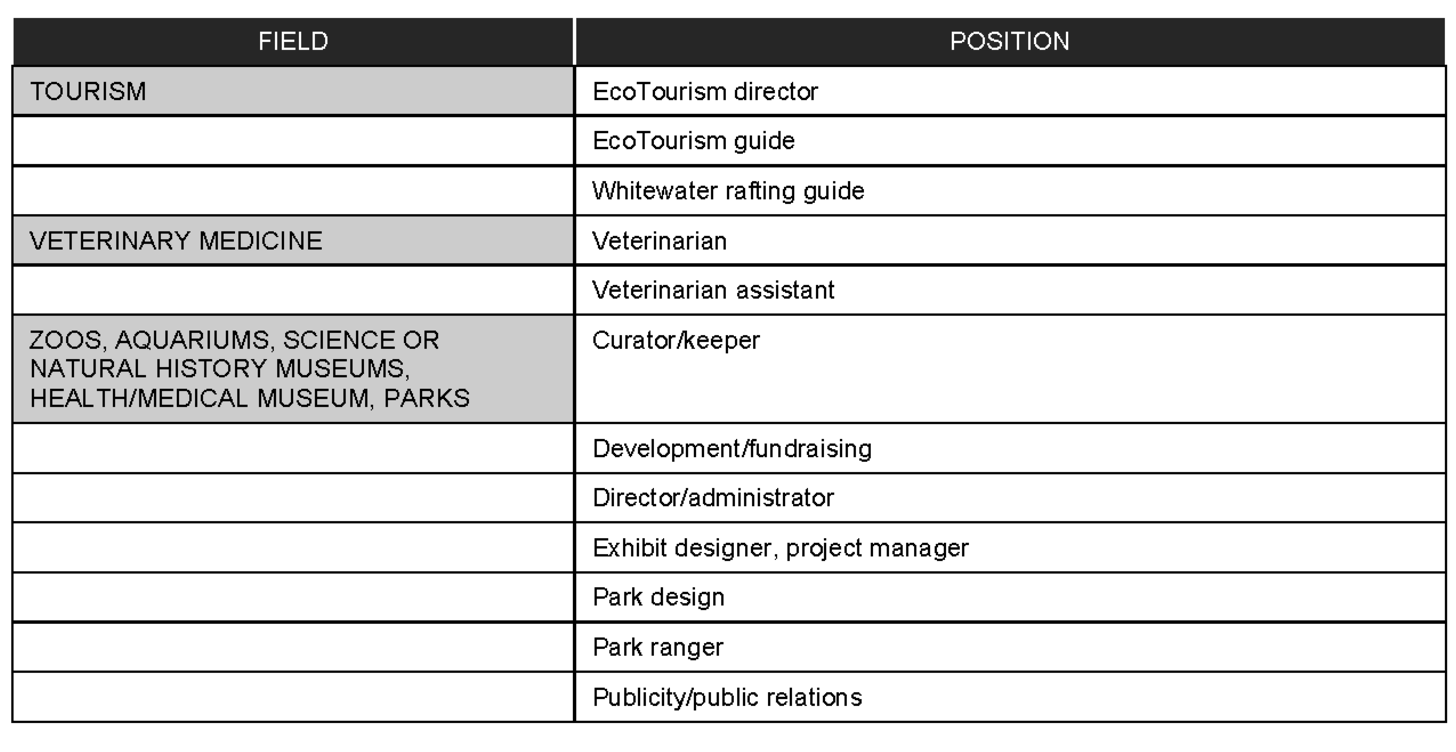
\includegraphics[page=1,width=\paperwidth]{./last-jobs-slide.pdf}}
\begin{frame}[plain]
\end{frame}
}

\section{How should you prepare for graduate school, professional school, or a
    job in industry?}

\begin{noheadline}
\begin{frame}[t]
\frametitle{How to prepare for graduate school, professional school, or a job
    in industry?}
    \vspace{-4mm}
    \begin{adjustwidth}{-1.5em}{-1.5em}
    \begin{flushleft}
        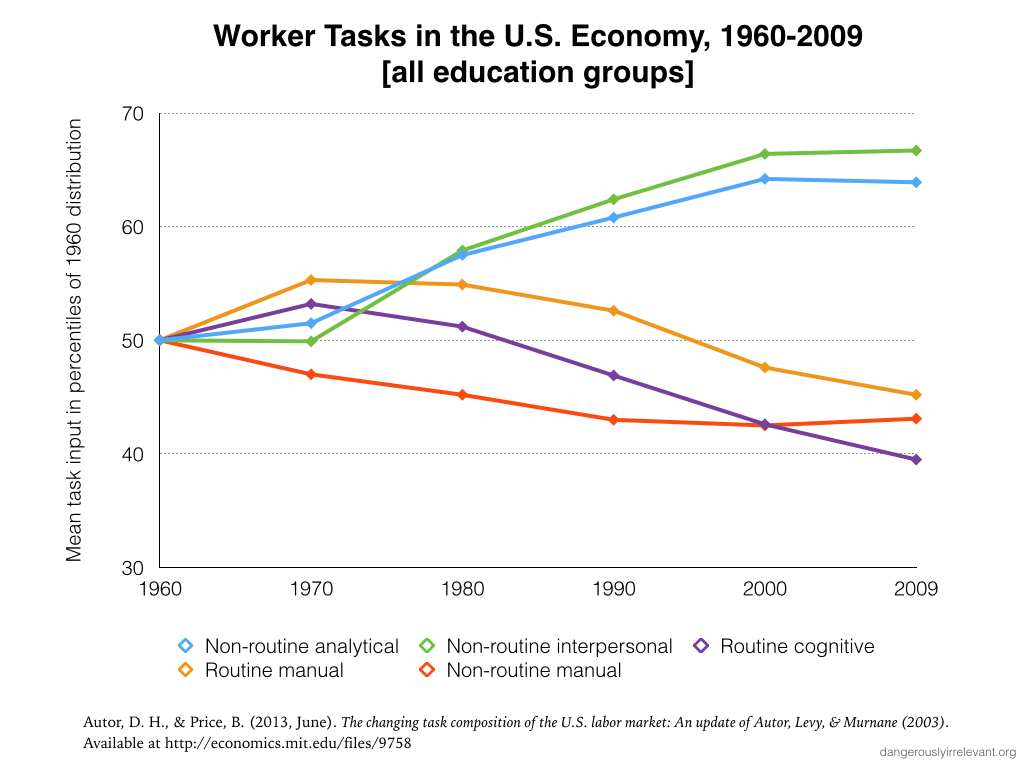
\includegraphics[page=1,width=0.96\textwidth]{../images/us-worker-task-plot.png}
    \end{flushleft}
    \end{adjustwidth}

    \note[item]{Study by economists at MIT}
    \note[item]{Label lines---show parents (late 1970s)---what's the
        punchline---what does it mean for you versus your parents}
    \note[item]{Top non-routine analytical and non-routine interpersonal}
    \note[item]{Routine and manual}
    \note[item]{TAKE HOME: Non-routine tasks becoming much more
        prevalent---Bloom's 1-2 = routine; Bloom's 3-6 = non-routine}
\end{frame}
\end{noheadline}

\begin{noheadline}
\begin{frame}[t]
    \begin{adjustwidth}{-1.5em}{-1.5em}
        From the sheets we passed out, what are the top 3 attributes of
        successful applicants?

        \nbox{Problem solving/intellectual potential; Ability to work with
            others; Maturity/emotional stability}
        
        \vspace{2cm}
        How will you get better at them?

        \nbox{In an interview, you have to have \highlight{data}!}
        \nbox{Seek out leadership positions}
    \end{adjustwidth}
\end{frame}
\end{noheadline}

\begin{noheadline}
\begin{frame}[t]
    \begin{adjustwidth}{-1.5em}{-1.5em}
        \begin{itemize}
            \item What is the role of your numbers (GPA, scores on
                DAT/MCAT/PCAT/GRE, etc.)?

                \nbox{They are baseline---It shows that you are good at school}

            \vspace{2cm}
            \item Why is the average age of matriculation to med school 25? Why
                has it been increasing recently?

                \nbox{Looking for individuals with greater emotional maturity,
                    perspective, and interpersonal skills}
        \end{itemize}
    \end{adjustwidth}
\end{frame}
\end{noheadline}

\begin{noheadline}
\begin{frame}[t]
    \begin{adjustwidth}{-1.5em}{-1.5em}
       The three most revealing interview questions:

       \begin{enumerate}
           \item What are you going to do to change the world?

               \nbox{Are you an original thinker and intellectual leader? Have
                   you thought deeply about the broader context of problems in
                   your field?}

               \vspace{1cm}
           \item Tell me about a book you have read recently and how it has
               changed you?

               \nbox{Do you immerse yourself in what you do and think
                   critically? Or are you just going through the motions? Are
                   you creative?}

               \vspace{1cm}
           \item Do you enjoy your own mind? And, if so, how?

               \nbox{Do you value independent intellectual growth and
                   curiosity}
       \end{enumerate}  
       \nbox{It helps to have experiences (data!) to talk about!}
    \end{adjustwidth}
\end{frame}
\end{noheadline}

\begin{noheadline}
\begin{frame}[t]
    \begin{adjustwidth}{-1.5em}{-1.5em}
        How should you go about getting letters of recommendation?

        \nbox{Letter writers have to describe how long they have known the
            applicant and in what capacity? You have to establish professional
            relationships with potential letter writers; you have to take the
            initiative to establish these relationships}
    \end{adjustwidth}
\end{frame}
\end{noheadline}

\end{document}

\clickerslide{
\begin{frame}
    \begin{clickerquestion}
        \item 
        \begin{clickeroptions}
            \item 
            \item 
            \item 
            \item 
        \end{clickeroptions}
    \end{clickerquestion}
\end{frame}
}
